% !TEX encoding = UTF-8
%Koma article
\documentclass[fontsize=12pt,paper=letter,twoside]{scrartcl}
\usepackage{float}
\usepackage{listings}
\usepackage{makecell}

%Standard Pre-amble
\usepackage[top=4cm,bottom=4cm,left=3cm,right=3cm,asymmetric]{geometry}
%\geometry{landscape}                % Activate for for rotated page geometry
%\usepackage[parfill]{parskip}    % Begin paragraphs with an empty line rather than an indent
\usepackage[table,xcdraw]{xcolor}
\usepackage{graphicx}

\usepackage{amsmath}
\usepackage{amssymb}
\usepackage{epstopdf}
\DeclareGraphicsRule{.tif}{png}{.png}{`convert #1 `dirname #1`/`basename #1 .tif`.png}
% Listings needs package courier
\usepackage{listings} % Needs 
\usepackage{courier}

\usepackage[framemethod=TikZ]{mdframed}
\usepackage{url}

\usepackage{sty/bsymb} %% Event-B symbols
\usepackage{sty/eventB} %% REQ and ENV
\usepackage{sty/calculation}

%Maths
\usepackage{amssymb,amsmath}
\def\Fl{\mathbb{F}}
\def\Rl{\mathbb{R}}
\def\Nl{\mathbb{N}}
\def\Bl{\mathbb{B}}
\def\St{\mathbb{S}}
\newcommand{\ovr}{\upharpoonright}
\newcommand{\var}[1]{\textit{#1}}
%Useful definitions
\newcommand{\mv}[1]{\textit{m\_#1}}
\newcommand{\cv}[1]{\textit{c\_#1}}
\newcommand{\degree}[1]{^{\circ}\mathrm{#1}}
%\newcommand{\comment}[1]{{\footnotesize \quad\texttt{--}\textrm{#1}}}
\newcommand{\im}[1]{i\texttt{-\!#1}}

\usepackage[headsepline]{scrpage2}
\pagestyle{scrheadings}
\ihead[]{\small EECS4312 Report1}
\ohead[]{\small \thepage}
\cfoot[]{}
\ofoot[]{}


%%%%PVS environment%%%%%%%%%%%%%%%%%%%
\lstnewenvironment{pvs}[1][]
    {\lstset{#1,captionpos=b,language=pvs,
    mathescape=true,
    basicstyle=\small\ttfamily,
    numbers=none,
    frame=single,
    % numberstyle=\tiny\color{gray},
    % backgroundcolor=\color{lightgray},
    firstnumber=auto
    }}
    {}
 %%%%%%%%%%%%%%%%%%%%%%%%%%%%%%%%
 
%%%%Verbatim environment%%%%%%%%%%%%%%%%%%%
\lstnewenvironment{code}[1][]
    {\lstset{#1,captionpos=b,
    mathescape=true,
    basicstyle=\small\ttfamily,
    numbers=none,
    frame=single,
    % numberstyle=\tiny\color{gray},
    % backgroundcolor=\color{lightgray},
    firstnumber=auto
    }}
    {}

% \newenvironment{boxed}[1]
%    {\begin{center}
%    #1\\[1ex]
%    \begin{tabular}{|p{0.9\textwidth}|}
%    \hline\\
%    }
%    { 
%    \\\\\hline
%    \end{tabular} 
%    \end{center}
%    }
 %%%%%%%%%%%%%%%%%%%%%%%%%%%%%%%%
 
 %Text in a box
\newenvironment{textbox}
    {\begin{center}
    \begin{tabular}{|p{0.9\textwidth}|}
    \hline\\
    }
    { 
    \\\\\hline
    \end{tabular} 
    \end{center}
    }

\usepackage{hyperref}

%Highlight \hl{}
\usepackage{soul}

\usepackage{enumitem}
\newlist{mylist}{itemize}{1}
\setlist[mylist]{label=\textbullet,leftmargin=1cm,nosep}

\usepackage{multirow}

% Reduce space between figure and caption
%\usepackage{caption}
%\captionsetup[table]{font=small,skip=0pt}     %% Adjust here
%or equivalently 
\usepackage[font=small,skip=4pt]{caption}
%Useful definitions
%\newcommand{\mv}[1]{\textit{m\_#1}}
%\newcommand{\cv}[1]{\textit{c\_#1}}
%\newcommand{\degree}[1]{^{\circ}\mathrm{#1}}
%\newcommand{\comment}[1]{{\footnotesize \quad\texttt{--}\textrm{#1}}}


%For Code Stylings
\usepackage{listings}
\usepackage{color}

\definecolor{dkgreen}{rgb}{0,0.6,0}
\definecolor{gray}{rgb}{0.5,0.5,0.5}
\definecolor{mauve}{rgb}{0.58,0,0.82}

\lstset{frame=tb,
  language=Java,
  aboveskip=3mm,
  belowskip=3mm,
  showstringspaces=false,
  columns=flexible,
  basicstyle={\small\ttfamily},
  numbers=none,
  numberstyle=\tiny\color{gray},
  keywordstyle=\color{blue},
  commentstyle=\color{dkgreen},
  stringstyle=\color{mauve},
  breaklines=true,
  breakatwhitespace=true,
  tabsize=3
}

% Set the header
\ihead[]{\small EECS4313 Assignment-2}


%%%%%%%%%%%%Enter your names here%%%%%%%%
\author{Student Name | Student Number | EECS Account
\and \textbf{Edward Vaisman | 212849857 | eddyv}
\and \textbf{Robin Bandzar | 212200531 | cse23028}
\and \textbf{Kirusanth Thiruchelvam | 212918298 | kirusant}
\and \textbf{Sadman Sakib Hasan | 212497509 | cse23152}
}
%%%%%%%%%%%%%%%%%%%%%%%%%%%%%%%%

\date{\today} % Display a given date or no date

\begin{document}
\title{EECS 4313 Assignment 2 \\Black-box and White-box Testing with JUnit}
\maketitle

\newpage

%%%%%%%%%%%%%%%%%%%%%%%%%%%%%%%
\tableofcontents


\newpage


%%%%Rest of your document goes here%%%%%%%%%%%%%%%%%%%

\section{Black Box Testing}
\begin{itemize}
\item \textbf{Technique}: \emph{Boundary Value Testing}
\item \textbf{Class}: \emph{net.sf.borg.common.SocketClient.java}
\item \textbf{Method}: \emph{sendMsg(String host, int port, String msg)}
\item \textbf{Method Description}:
This method sends a given message to a given host, port and returns the response from the socket.
\begin{itemize}
\item the first argument \emph{host} is the host that the socket client should be connected to.
\item the second argument \emph{port} is the port on the host that the socket client should be connected to
\item the third argument \emph{msg} is the message that should be sent over the host and port given.
\end{itemize}
\begin{description}
\item[IOException:] If an I/O error occurs when sending the message.
\end{description}
\item \textbf{Justification}: Boundary value testing is best suited for methods that have inputs that could be seperated into partitions. For this method the port could be partitioned. We have our valid partition which is between 0 and 65535 (inclusive) and our invalid partitions which is any port\textless 0 or any port\textgreater 65535. The msg could be anything and the host could be partitioned into valid/invalid hostnames.
\item \textbf{Evaluation}: The test below applies weak robust testing on the method \emph{sendMsg} which reveals a bug within the method that causes the method to throw an \\ \mbox{IllegalArgumentException} If the port parameter is outside the specified range of valid port values, which is between 0 and 65535, inclusive. Refer to Figure.~\ref{fig:bbt_bvt1}, Figure.~\ref{fig:bbt_bvt2} and Listing ~\ref{list:weak_robust}\\ \\
The test is designed to not fail on any  \mbox{IOExceptions} that may occur such as \mbox{UnknownHostException} or \mbox{ConnectionException} since the method is supposed to \emph{throw} an \mbox{IOException}. \\ \\
However, applying weak normal testing will cause all the tests to pass. Refer to Figure,~\ref{fig:bbt_bvt3} and Listing.~\ref{list:weak_normal}
\newpage
\begin{lstlisting}[caption={Weak Robust Testing Variables},label={list:weak_robust}]
String validHost = "localhost";
port_norm = 2929; // x_norm
port_min = 0; // x_min
port_min_plus = 1; // x_min+
port_max = 65535; // x_max
port_max_minus = 65534; // x_max-
// robustness
String invalidHost = "asdfasdf"; //unknownhostexception
int port_min_minus = -1; // x_min-
int port_max_plus = 65536; // x_max_+

\end{lstlisting}

\begin{lstlisting}[caption={Weak Normal Testing Variables},label={list:weak_normal}]
String validHost = "localhost";
port_norm = 2929; // x_norm
port_min = 0; // x_min
port_min_plus = 1; // x_min+
port_max = 65535; // x_max
port_max_minus = 65534; // x_max-
\label{list:weak_normal}
\end{lstlisting}
\newpage
\begin{figure}[!htb]
\begin{center}
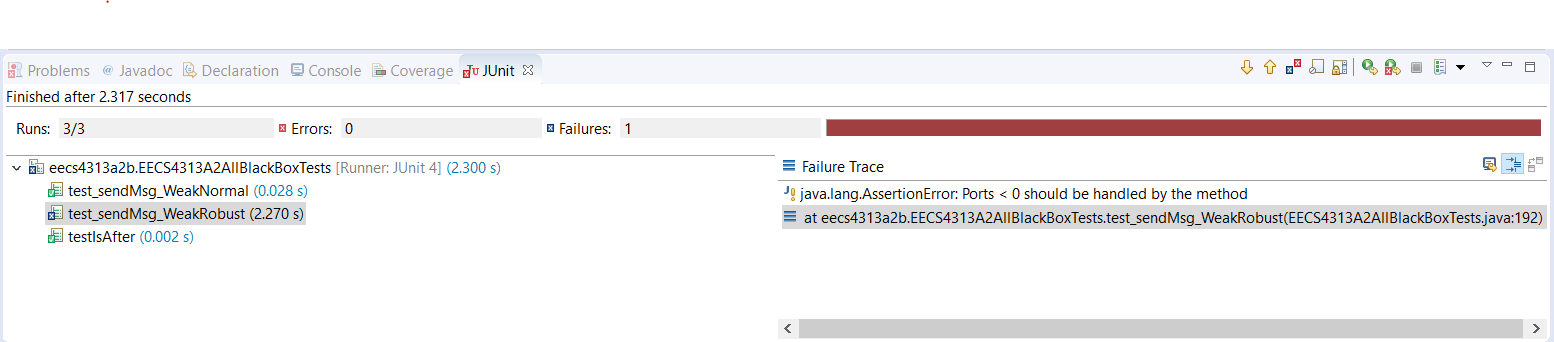
\includegraphics[width=.99\textwidth]{images/bbt/bvt-fail-1.png}
\end{center}
\caption{Test results using Weak Robust Boundary Value Testing}
\label{fig:bbt_bvt1}
\end{figure}

\begin{figure}[!htb]
\begin{center}
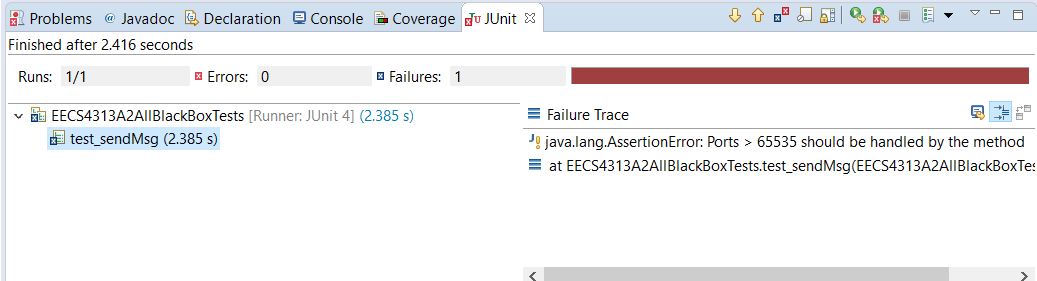
\includegraphics[width=.99\textwidth]{images/bbt/bvt-fail-2.png}
\end{center}
\caption{Test results using Weak Robust Boundary Value Testing}
\label{fig:bbt_bvt2}
\end{figure}

\begin{figure}[!htb]
\begin{center}
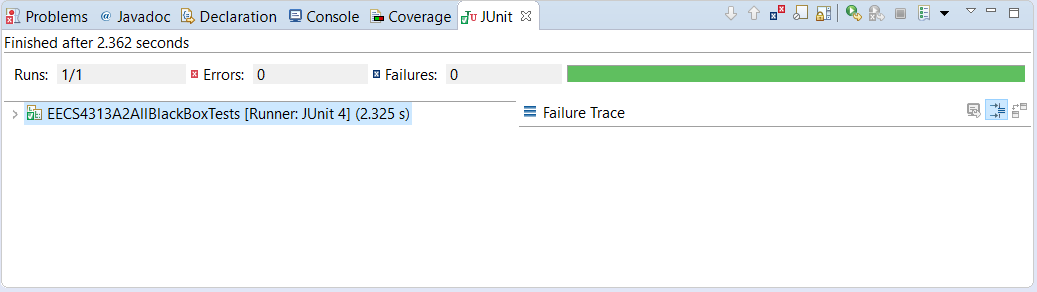
\includegraphics[width=.99\textwidth]{images/bbt/bvt-pass.png}
\end{center}
\caption{Test results using Weak Normal Boundary Value Testing}
\label{fig:bbt_bvt3}
\end{figure}

\newpage
\begin{lstlisting}
public class EECS4313A2AllBlackBoxTests implements SocketHandler {

	/**
	 * process a socket message
	 */
	@Override
	public synchronized String processMessage(String msg) {
		return msg;
	}

	@Test
	public void test_sendMsg() {
		/** Method used: Boundary Value Testing **/
		String validHost = "localhost";

		int port_norm = 2929; // x_norm
		int port_min = 0; // x_min
		int port_min_plus = 1; // x_min+
		int port_max = 65535; // x_max
		int port_max_minus = 65534; // x_max-

		// robustness
		String invalidHost = "asdfasdf";
		int port_min_minus = -1; // x_min-
		int port_max_plus = 65536; // x_max_+

		String response = "";
		// port_norm
		String msg = "Port 2929";
		SocketServer ss = new SocketServer(port_norm, this);
		try {
			response = SocketClient.sendMsg(validHost, port_norm, msg);
			assertTrue("Testing if a localhost on port_norm sends a message", response.equals(msg));
		} catch (IOException e) {
			e.printStackTrace();
		}
		/* Unknown host exception extends IOException */
		try {
			response = SocketClient.sendMsg(invalidHost, port_norm, msg);
			assertTrue("Testing if an invalid host on port_norm sends a message", response.equals(msg));
		} catch (IOException e) {
			e.printStackTrace();
		}

		// port_min
		/*
		 * Throws connection problem. port 0 isn't available on my computer Connect
		 * Exception extends Socket Exception which extends IOException
		 */
		msg = "Port 0";
		try {
			ss = new SocketServer(port_min, this);
			response = SocketClient.sendMsg(validHost, port_min, msg);
			assertTrue("Testing if a localhost on port_min sends a message", response.equals(msg));
		} catch (IOException e) {
			e.printStackTrace();
		}
		// port_min+
		msg = "Port 1";
		try {
			ss = new SocketServer(port_min_plus, this);
			response = SocketClient.sendMsg(validHost, port_min_plus, msg);
			assertTrue("Testing if a localhost on port port_min+ sends a message", response.equals(msg));
		} catch (IOException e) {
			// TODO Auto-generated catch block
			e.printStackTrace();
		}

		// port_max
		msg = "Port 65535";
		try {
			ss = new SocketServer(port_max, this);
			response = SocketClient.sendMsg(validHost, port_max, msg);
			assertTrue("Testing if a localhost on port port_max sends a message", response.equals(msg));
		} catch (IOException e) {
			// TODO Auto-generated catch block
			e.printStackTrace();
		}

		// port_max-
		msg = "Port 65534";
		try {
			ss = new SocketServer(port_max_minus, this);
			response = SocketClient.sendMsg(validHost, port_max_minus, msg);
			assertTrue("Testing if a localhost on port_max- sends a message", response.equals(msg));

		} catch (IOException e) {
			// TODO Auto-generated catch block
			e.printStackTrace();
		}

		// port_min-
		/*
		 * Illegal argument Exception
		 */

		msg = "Port -1";
		try {
			ss = new SocketServer(port_min_minus, this);
			response = SocketClient.sendMsg(validHost, port_min_minus, msg);
			assertTrue("Testing if a localhost on port_min- sends a message", response.equals(msg));
		} catch (IOException e) {
			e.printStackTrace();
		} catch (IllegalArgumentException iae) {
			fail("Ports < 0 should be handled by the method");
		}

		// port_max+
		/*
		 * Illegal argument Exception
		 */
		msg = "Port 65536";
		try {
			ss = new SocketServer(port_max_plus, this);
			response = SocketClient.sendMsg(validHost, port_max_plus, msg);
			assertTrue("Testing if a localhost on port_max+ sends a message", response.equals(msg));
		} catch (IOException e) {
			e.printStackTrace();
		} catch (IllegalArgumentException iae) {
			fail("Ports > 65535 should be handled by the method");
		}
	}

}
\end{lstlisting}
\end{itemize}
\newpage
\section{White Box Testing}

\begin{itemize}
\item The statement coverage measurements for your Assignment 2 test suite.
\item A description of the test cases that you added in this assignment to improve statement
coverage. The marker will not read your code in order to see what you tested. You have to
describe it.
\item The statement coverage measurements for your final submission. Include the screenshots of
the test running results and the screenshots of the coverage measurement. If your coverage is
not 100%, include a discussion on why that is.
\item The Control Flow Graph you created. Indicate the segments clearly (you will probably need
to include the code for this).
\item The path coverage discussion described in section 2 above.
\item Attaching bug reports if bugs are discovered using your testing methods. You should use the
same bug report format as in Assignment 1. Do not file these bug reports to the project’s bug
report system.
\item An appendix with the specification of the methods you are testing (if there are new ones). 
\end{itemize}

\end{document}
